\ifdefined\XeTeXrevision\else\pdfoutput=1\fi
\documentclass[11pt]{article}
\usepackage[margin=1in]{geometry}
\usepackage{booktabs}
\usepackage{amsmath}
\usepackage{graphicx}
\usepackage{xcolor}
\usepackage{hyperref}
\usepackage{microtype}
\hypersetup{colorlinks=true, linkcolor=blue!60!black, citecolor=blue!60!black,
  urlcolor=blue!60!black, pdftitle={The Want and the Way},
  pdfauthor={Franci Penov}}
\title{The Want and the Way:\\One Door for What, One Door for How}
\author{Franci Penov \\ kortexa.ai \\ \texttt{francip@kortexa.ai}}
\date{2026-08-20}

\begin{document}
\maketitle

\begin{abstract}
The resident-referent note~\cite{penov2026inside} showed a want can
live inside a frozen model; the goal-pursuit ladder before it showed
the program's conditioning bus encodes a want's object but barely acts
on it. This note resolves that tension as a question of DOORS. Seven
registered cells, two scales. The door test: the same 230M errand, the
same want, the same drive --- entering through a latent prefix the
referent moves the submit by +0.52 over the crossed
base, 80\% of the text ceiling
(+0.65), while through the bus it moves it by
+0.11; symbols act at the door where language enters.
Asked instead for a MANNER --- look around, or open things --- the bus
is fluent: the counter-habitual focus lifts first-tick opening from
0.00 to 0.87,
wins 52 and loses 0 of 60 paired first ticks
against the swapped packet, and the same phrasing as prompt text does
nothing (0.00); at 230M the latent
channel is the only door direction fits through. The grip is total,
though: under the LOOK packet every decision point of every episode is
a look, and delivery fraction is no dial --- a seed-dependent phase
edge with the errand-ending act never returning --- whereas rotating
the packet toward its own drive baseline at constant strength releases
it smoothly (look share 1.00\,$\to$\,0.79,
done recovering to 0.26). Strength is binary,
direction is graded. At 27B the grip is gone natively: a frozen
Qwen3.8-27B tolerates the full dose the small family cannot, reads the
focus linearly at every depth, and LEANS --- open share
0.24\,$\to$\,0.68
with the errand still ending (done 0.13), the bus door
matching instruction text (0.683 vs
0.672) without any instruction. Then
both doors at once: the goal through the prefix, the manner through
the bus, on the frozen 27B --- the mix swings to the focused tool
(open 0.20\,$\to$\,0.70)
while the errand completes at prefix-only's level (0.9 /
1.0 / 0.8), the
cost of style paid in ticks, the doors physically disjoint. In one
sentence, honestly flagged as an analogy: tell a big-enough model what
you want at the front door and how you want it done through the side
door, and it does both --- a small one can only be told how, and then
cannot stop.
\end{abstract}

\section{Two doors, two questions}

Every want in this program has to enter a frozen model somewhere.
The goal-pursuit ladder~\cite{penov2026hostblock,penov2026act} put
wants through the conditioning bus --- a 256-dimensional packet
injected into the residual stream at three depths --- and found a
split: a linear head reads the goal's object out of the packet at
0.69--0.81 against chance 0.125, yet naming an item in the packet
moves the submit by only $+0.18$. The loss is at the readout. The
resident-referent note~\cite{penov2026inside} then carried a goal
LINE through a different door, as embeddings in a prefix slot, and
errand success sat at the text ceiling --- but success alone can ride
chain preference plus generic drive, which is exactly how the bus
fooled its first readouts. Two questions follow and this note answers
both. First: is the symbol-readout failure a property of the WANT or
of the DOOR? Second: if the bus is the wrong door for a what, is it the
right door for a how --- and what does a frozen model do when the what
and the how arrive through different doors at once?

The setting throughout is the G1 errand: a chain of three places, a
two-item reveal, a budget of eight ticks, three tools (\texttt{look},
\texttt{open}, \texttt{done}), ten evaluation chains, greedy decode.
The small host is LFM2.5-230M with the creature's production
self-block armed; the large host is Qwen3.8-27B. Every cell was
registered with its readings stated before it ran; the registrations
and their dates are in the track plan.

\section{The door was the bottleneck}

G6 puts the SAME want through both doors with the crossed probe that
exposed the bus: every evaluation chain is run against every one of
the eight installed items, so the chain's own preference is held fixed
while the installed referent moves. The decisive cell installs the
DISTRACTOR's referent and asks whether the model submits it more often
than when an out-of-pair item is installed (Table~\ref{tab:doors}).
Through the text door the lift is +0.65
(1.00 vs 0.35), the ceiling.
Through the prefix door --- the goal line embedded by the model's own
input table, prepended to a goal-free prompt, no text anywhere, no
bridge ever trained on prefixed inputs --- it is +0.52
(0.79 vs 0.27). Through
the bus it is +0.11 (0.41 vs
0.31), reproducing the earlier $+0.16$ on a new
device. Same want, same model, same drive: moved from the bus to the
prefix, symbol-level readout goes from barely there to
80\% of the text ceiling. Plain
success tells the same story (1.00/1.00/1.00
prefix against 0.70/0.70/0.70 bus, three seeds).
The readout works at the door where symbols enter the stream the way
language does.

Two further cells bound the claim. When the two doors DISAGREE ---
prefix naming the target, bus naming the distractor, and the reverse
--- neither dominates: at the two seeds where the doors compose the
prefix wins 20, the bus 19
(1 other), and whichever door names the target wins
about 0.6 both ways; the chain's own preference casts the deciding
vote. And at the third seed the two channels together push the decode
out of the tool-call format entirely --- 20
of 20 conflict cells decided nothing, success 0.00 --- while each door
works alone. Two channels can interfere the way two blocks
do~\cite{penov2026onestage}; one seed of three, recorded as the
composition law's first sighting at the channel level.

\section{The bus's demonstrated job is the how}

If the bus is a poor door for nouns, GF asks it for what it has done
well everywhere else in the program: a direction. The focus alphabet is
two manners, LOOK (``keep looking around'') and OPEN (``open things''),
one-to-one with the errand's tool families; the errand runs
goal-FREE so direction is measured uncontaminated by goal content.
Per seed a focus bridge and a constant (drive-only) bridge are trained
by the standing recipe; the evaluation packets come from held-out
phrasings only. Four arms: the focus packet, the SWAPPED packet (with
two focuses the derangement is total), no focus (the drive alone ---
the habit), and the focus as text in the prompt (the registered
ceiling). The preregistered metrics are distributional only: the
first-tick focused-tool rate paired focus-vs-swapped per chain (the
one tick where context is identical across arms by construction), and
the whole-episode tool mix with its Jensen--Shannon divergence
focus-vs-swapped, signed by whether the focused tool's share rises
under the true packet. The mix carries a fourth category,
\texttt{other}, for replies that parsed to no tool, so an
incoherent decode cannot silently renormalize toward whatever little
parsed.

Both primaries, both focuses, every seed (Table~\ref{tab:focus230}).
The habit is deterministic, 0.50/0.25/0.25
look/open/done, and never opens first. Under the OPEN packet first-tick
opening goes 0.00\,$\to$\,0.87
and the open share 0.25\,$\to$\,0.79;
under the LOOK packet the mix is 1.00/0.00/0.00 at every decision
point of every episode. Paired first ticks: 52 wins, 0 losses,
8 ties pooled over both focuses; signed JS +0.69.
The registered ceiling was not one: the same held-out phrasing placed
in the prompt over the same drive does approximately nothing
counter-habitual --- first-tick open 0.00
at every seed, open share 0.22 against
the habit's 0.25. At 230M, in this world,
instruction text does not direct and the bus outperforms language at
the bus's demonstrated job. Every prior rung had text as the ceiling
the latent chased; here the latent channel is the only door direction
fits through. The channel carries the HOW, not the WHAT.

\section{Strength is binary, direction is graded}

GF left one observation that made composition look doomed: at the
trained dose the LOOK packet does not bias the mix, it owns it, and
\texttt{done} never fires. A focus that prevents every other act is
a compulsion, not a preference. GF-2 swept the one obvious knob, the
generate-time delivery fraction, from the trained 0.15 down by a
factor of ten, with a registered selector for a usable bias band
(focused share $\le 0.85$, done share $\ge 0.05$). The selector
returns null. Pooled look share by dose reads
1.00/0.54/0.51/1.00/0.95/0.79 --- non-monotone, full possession reviving at
0.05 after a dip --- and done under the LOOK packet is 0.000 at every
dose. The dip is not a middle (Figure~\ref{fig:arc}b): per-seed
shares at dose 0.1 are 0.66/0.00/0.96, at 0.075
0.20/0.33/1.00, at 0.05 1.00/1.00/1.00. Individual
cells sit at possession or at nothing; the pooled intermediate values
average a bimodal collapse whose edge moves with seed and focus.
Direction never flips --- signed JS stays positive at every dose ---
its grip just switches between total and absent. This is the
program's dose-brittleness law, first seen in content margins,
measured here behaviorally: delivery fraction is a phase dial.

GF-2b asked whether a lean could be CONSTRUCTED instead, by rotating
the focus packet toward the constant (drive-only) packet at the full
trained dose, with the merging negative~\cite{penov2026onestage} as
the recorded risk prior --- that arc found two content packets destroy
each other, but content mixed with its own drive is a structure no
prior negative tested. Two loci. Mixed in FEATURE space, before the
bridge, nothing arrives: all three alphas reproduce the unmixed anchors
to three decimals (look 1.00, open 0.786, JS
0.6875) because the bridge's source-statistics normalization
absorbs the interpolation before it reaches the packet. Mixed in
PAYLOAD space, on the per-layer deltas, there is a real dial
(Figure~\ref{fig:arc}c): look share 1.00/0.98/0.79, open share
0.60/0.36/0.26 across alpha 0.75, 0.5, 0.25, done recovering
to 0.26 under the OPEN packet, JS decaying smoothly
(0.49/0.42/0.12) and never changing sign, per-seed spreads graded
rather than 0-or-1. The registered per-focus selector passes at alpha
0.25. The injection renormalizes, so alpha steers the packet's
direction at constant delivered strength --- which is what licenses
the synthesis: the channel's grip is all-or-nothing in how hard it
pushes and continuous in where it points. Mixing a focus with its own
drive composes gracefully where two rival contents destroyed each
other.

\section{At 27B the grip becomes a lean}

The scale-promotion rule of the program is that a creature-scale
result is a stepping stone until it reappears on a host worth serving.
The first rung is the doors themselves: the focus and constant bridges
trained against a frozen Qwen3.8-27B in 23 minutes,
every gate at ceiling (held-out phrasing accuracy 1.00/1.00, auxiliary
head 4/4, zero-dose decode token-identical, base weights byte-identical
at every boundary). Two observations came free. The coherence gate ---
one untrained constant-state feed must not decohere greedy decode ---
PASSED at the full dose with zero halvings; the same feed word-salads
the small family. The severity of the dose-decoherence law is
host-dependent. And the tap scan could not discriminate: a linear probe
reads the focus at 1.0 on train and held-out at all eight depths
scanned (layers 3--59 of 64), so the
tie-break chain resolved to the recorded prior at layer 51; the
two-focus signal is linearly readable everywhere in the 27B.

The behavioral eval then ran GF's design on those doors
(Table~\ref{tab:focus27}). The counter-habitual cell carries it:
under the OPEN packet the 27B's open share goes
0.24\,$\to$\,0.68,
first-tick open 0.3\,$\to$\,0.8,
paired against the swapped packet 8--0--2
--- and \texttt{done} stays alive at 0.13, \texttt{look}
present at 0.18. The errand
still ends; the repertoire is intact; the packet LEANS the model. The
LOOK packet reads the same way on an already look-heavy habit
(first-tick 0.7\,$\to$\,1.0,
share 0.60\,$\to$\,0.62,
done 0.19). Nothing approaches the 230M's 1.00-share
capture: same bank, same recipe, same dose --- the grip is a property
of the host scale, not of the channel. The text arm flips too: the
focus as prompt text works at 27B (open share
0.67), and the trained bus door matches
it (0.683 vs 0.672;
look 0.615 vs 0.600).
At 27B the latent channel buys instruction-following strength without
instruction text, which is the door's whole value proposition, now
measured at the scale that matters. The signed JS is 0.20
against the 230M's 0.69 precisely because this is a lean and
not a grip. One door seed; the ten chains are the replication axis;
278 decodes, zero think-blocks stripped, zero parse
fallbacks --- the 27B plays the errand's JSON natively.

\section{Wants with style}

GF-3 is the rung the arc was built for: the goal through the prefix
door and the manner through the bus, simultaneously, in the errand
WITH goals, on the frozen 27B. The venue is native because the lean is
intrinsic there, so the composition claim carries no alpha-machinery
caveat. Three arms over the ten chains: prefix only (the goal line as
latent prefix plus the constant packet --- also the first measurement
of the prefix door carrying a goal at 27B), prefix plus the LOOK
packet, prefix plus the OPEN packet. Congruence is not pre-labeled;
both tools are instrumental to the errand and which focus helps is the
question. Because the two doors had never shared one generate call,
three plumbing gates were registered and all passed: hooks armed at
zero dose are token-identical to a plain decode with and without the
prefix, and the per-chain prefix length is constant across arms so the
injection lands at the same place in every arm. The doors are
physically disjoint --- the injection touches only the final prompt
position and each generated token; the prefix is read through
attention, never written.

The precondition passed with headroom: prefix-only success
0.9 from a purely latent referent.
Then style with substance (Table~\ref{tab:gf3},
Figure~\ref{fig:arc}d). Under the OPEN packet the mix swings hard ---
open 0.20\,$\to$\,0.70
of all decision points, first-tick open
0.2\,$\to$\,0.8
--- while the errand completes: success 0.8,
done alive at 0.13. Under the LOOK packet
success is 1.0, first-tick look
0.8\,$\to$\,1.0.
Paired per chain against prefix-only, LOOK helps 1,
hurts 0, same 9; OPEN helps
0, hurts 1, same 9. The
cost of style is ticks, not goals: +0.44
and +0.75 mean ticks-to-success. Single-
chain deltas at ten chains, stated as such; 135 seconds of
decode, zero parse fallbacks.

\begin{table}[t]
\centering
\small
\setlength{\tabcolsep}{4pt}
\begin{tabular}{lllrrr}
\toprule
 & & & \multicolumn{3}{c}{P(submit = distractor)} \\
door & success & follow installed & installed & elsewhere & lift \\
\midrule
text & 1.00/1.00/1.00 & 1.00/1.00/1.00 & 1.00 & 0.35 & +0.65 \\
prefix-only & 1.00/1.00/1.00 & 0.89/0.90/0.89 & 0.79 & 0.27 & +0.52 \\
bus-only & 0.70/0.70/0.70 & 0.60/0.50/0.61 & 0.41 & 0.31 & +0.11 \\
split-door & 0.80/0.90/0.00 & 0.63/0.75/-- & 0.53 & 0.34 & +0.19 \\
\bottomrule
\end{tabular}
\caption{G6 at 230M, three seeds (42/1042/2042). Success and
follow-installed-when-in-pair per seed; the causal cell pools decided
probe rows across seeds: installing the distractor's referent against
installing an out-of-pair item. The prefix door reaches
80\% of the text ceiling; the bus
door 17\%. Split-door at seed 2042
decided nothing (the channel-composition failure).}
\label{tab:doors}
\end{table}

\begin{table}[t]
\centering
\small
\setlength{\tabcolsep}{4pt}
\begin{tabular}{llrrrrlr}
\toprule
focus & arm & first tick & share & done & other & paired W--L--T & JS \\
\midrule
LOOK & habit & 1.00 & 0.50 & 0.25 & 0.00 &  &  \\
LOOK & packet & 1.00 & 1.00 & 0.00 & 0.00 & 26--0--4 & +0.69 \\
LOOK & shuffled & 0.13 & 0.14 & 0.01 & 0.06 &  &  \\
LOOK & text & 1.00 & 0.65 & 0.14 & 0.00 &  &  \\
OPEN & habit & 0.00 & 0.25 & 0.25 & 0.00 &  &  \\
OPEN & packet & 0.87 & 0.79 & 0.01 & 0.06 & 26--0--4 & +0.69 \\
OPEN & shuffled & 0.00 & 0.00 & 0.00 & 0.00 &  &  \\
OPEN & text & 0.00 & 0.22 & 0.18 & 0.08 &  &  \\
\bottomrule
\end{tabular}
\caption{GF at 230M, pooled over three seeds (30 episodes per arm).
First-tick focused-tool rate, focused-tool share of all decision
points, done and other shares, the paired first-tick record
focus-vs-swapped, and the signed JS divergence. The packet captures;
the text does nothing counter-habitual.}
\label{tab:focus230}
\end{table}

\begin{table}[t]
\centering
\small
\setlength{\tabcolsep}{4pt}
\begin{tabular}{llrrrrlr}
\toprule
focus & arm & first tick & share & done & other & paired W--L--T & JS \\
\midrule
LOOK & habit & 0.70 & 0.60 & 0.16 & 0.00 &  &  \\
LOOK & packet & 1.00 & 0.62 & 0.19 & 0.00 & 8--0--2 & +0.20 \\
LOOK & shuffled & 0.20 & 0.18 & 0.13 & 0.00 &  &  \\
LOOK & text & 1.00 & 0.60 & 0.20 & 0.00 &  &  \\
OPEN & habit & 0.30 & 0.24 & 0.16 & 0.00 &  &  \\
OPEN & packet & 0.80 & 0.68 & 0.13 & 0.00 & 8--0--2 & +0.20 \\
OPEN & shuffled & 0.00 & 0.19 & 0.19 & 0.00 &  &  \\
OPEN & text & 0.90 & 0.67 & 0.15 & 0.00 &  &  \\
\bottomrule
\end{tabular}
\caption{The same design on the frozen 27B, one door seed (10
episodes per arm). The packet leans --- done stays alive --- and the
bus door matches the text arm it could not touch at 230M.}
\label{tab:focus27}
\end{table}

\begin{table}[t]
\centering
\small
\setlength{\tabcolsep}{4pt}
\begin{tabular}{lrrrrlr}
\toprule
arm & success & finish tick & first look/open & look/open/done & helps/hurts/same & $\Delta$ticks \\
\midrule
prefix only & 0.90 & 5.11 & 0.8/0.2 & 0.63/0.20/0.17 & --- & --- \\
prefix + LOOK & 1.00 & 5.60 & 1.0/0.0 & 0.64/0.18/0.18 & 1/0/9 & +0.44 \\
prefix + OPEN & 0.80 & 5.88 & 0.2/0.8 & 0.17/0.70/0.13 & 0/1/9 & +0.75 \\
\bottomrule
\end{tabular}
\caption{GF-3 at 27B: the goal in the prefix, the manner on the bus,
ten chains. Success holds at prefix-only's level while the mix and the
first tick follow the packet; the paired columns compare each packet
arm against prefix-only chain by chain (ticks over chains both arms
solved).}
\label{tab:gf3}
\end{table}

\begin{figure}[t]
\centering
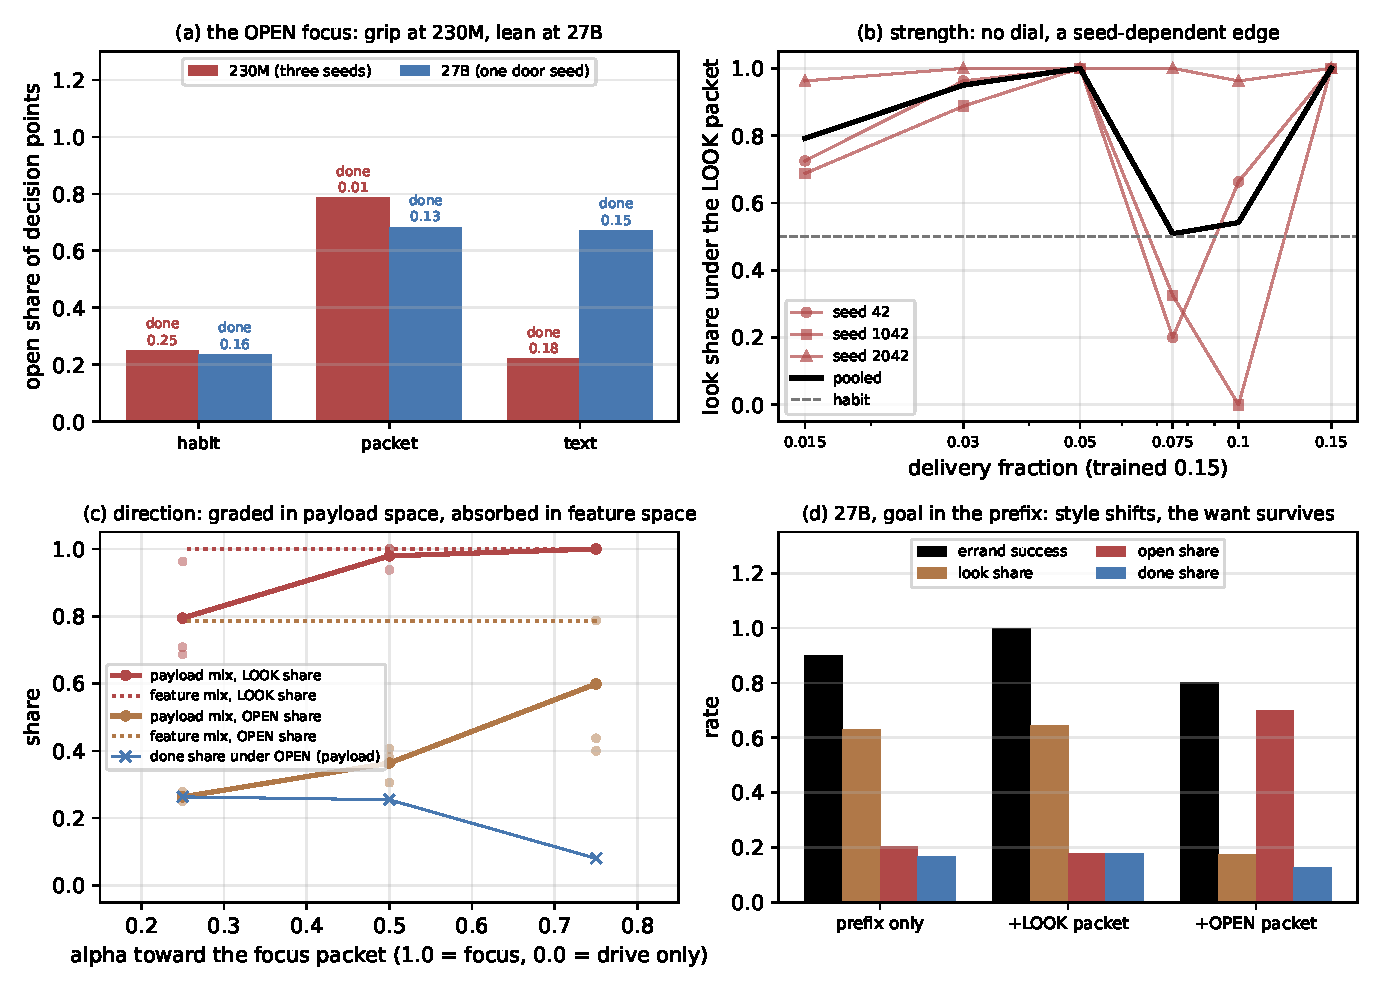
\includegraphics[width=\linewidth]{want-and-way.pdf}
\caption{(a) The OPEN focus's open share by arm: at 230M the packet
grips where text does nothing; at 27B packet and text agree and the
errand still ends. (b) GF-2: per-seed look share under the LOOK packet
against delivery fraction --- cells sit at possession or nothing, the
pooled curve is a bimodal average. (c) GF-2b: rotating the packet
toward its drive baseline at constant strength releases the grip
smoothly in payload space and not at all in feature space. (d) GF-3:
with the goal resident in the prefix, each packet moves the 27B's mix
toward its tool while success stays at the prefix-only level.}
\label{fig:arc}
\end{figure}

\section{What stands}

A want has a what and a how, and on a frozen model they want different
doors. The what --- a referent, a symbol --- acts when it enters where
language enters: the prefix door reaches 80\%
of the text ceiling on causal symbol-following where the bus reaches
17\%, with the same want, model, and
drive. The how --- a manner, a direction --- is the bus's job, and at
230M the bus is the only door it fits through, with total capture at
the trained dose, no volume knob on delivery strength, and a smooth
dial only on the packet's direction. At 27B the capture is gone
natively: the host tolerates the full dose, reads the focus at every
depth, and leans instead of gripping, the bus door now equal to
instruction text without any text. And the two doors compose on the
frozen 27B: the goal resident in the prefix, the manner on the bus,
behavior taking the style while the want survives. The program's
arbitration thesis~\cite{penov2026onestage} --- one stage, one act
--- gains its first two-door positive at the scale the promotion
principle names, with the mechanism that makes it clean: the doors
never touch the same position. The bounds are the usual ones and are
stated where they bind --- one door seed at 27B with chains as the
replication axis, ten chains per cell, a channel-composition failure
at one of three 230M seeds --- and the scale story cuts the other way
for the small host: it can be told how, and then cannot stop.

\section*{Addendum (2026-08-20): the replication arm at 230M}

The composition rung's optional replication arm ran the same day the
note was compiled: the split-door errand at 230M with GF-2b's
constructed lean (alpha 0.25) and, beside it, the unmixed grip, three
bridge seeds. Its registered precondition FAILED: prefix-only success
is 0.63 (0.7/0.8/0.4) against the 0.80
floor --- the same zero-shot prefix door that G6 measured at 1.00 at
every seed, now over GF's constant bridge (trained from the focus
exchange in the goal-free world) instead of G1's (trained from the
goal exchange). The door's readout depends on the drive packet beneath
it; a zero-shot door over one drive bridge is not a zero-shot door
over another. Underneath that, recorded against the weakened baseline:
neither lean composes (success 0.33 and
0.40 under LOOK and OPEN, the mix barely moving,
look 0.49\,$\to$\,0.56,
open 0.23\,$\to$\,0.24),
and both grips override exactly as GF-2 predicted (LOOK grip success
0.00 with look at 0.95
and done at 0.00; OPEN grip
0.03 with open at 0.90).
Two bounds tighten at once. The two-door composition is
host-scale-dependent on the evidence in hand: at creature scale any
packet on the bus taxes the resident want, graded by how far it points
from the drive, and the want never gets style for free. And the prefix
door's independence from the bus, implicit in Section~2, holds only
over the drive it was measured with. The clean separation of the two
--- GF-3r under G1's constant bridge --- is named in the track plan and
not run. Artifact \texttt{findings/goal-pursuit-gf3r-230m.json}.

\section{Reproducibility}

Every number renders from the bundled artifacts; the figure and tables
are generated by this note's renderer with assertions on the headline
claims. Registrations and results, dated before their runs, live in
\texttt{tracks/goal-pursuit/PLAN.md} (G6, GF, GF-2, GF-2b, the
GF-27B bridge and eval, GF-3); artifacts under
\texttt{findings/goal-pursuit-g6-230m.json},
\texttt{findings/goal-pursuit-gf*.json} carry every episode trace,
probe row, gate transcript, and checkpoint hash. The 27B door
checkpoints are pinned by sha256 in the bridge artifact and verified
before every decode that consumed them.\par

\begin{thebibliography}{9}
\bibitem{penov2026inside} F.~Penov. The Want That Lives Inside.
Preprint, 2026. \url{https://github.com/kortexa-ai/legolm.basis}.
\bibitem{penov2026act} F.~Penov. The Want Becomes the Act. Preprint,
2026. \url{https://github.com/kortexa-ai/legolm.basis}.
\bibitem{penov2026hostblock} F.~Penov. The Host Is Part of the Block.
Preprint, 2026. \url{https://github.com/kortexa-ai/legolm.basis}.
\bibitem{penov2026onestage} F.~Penov. One Stage, One Act. Preprint,
2026. \url{https://github.com/kortexa-ai/legolm.basis}.
\bibitem{lfm2026} Liquid AI. LFM2.5 model family. Model releases,
2025--2026. \url{https://huggingface.co/LiquidAI}.
\bibitem{qwen2026} Qwen Team. Qwen3.5--3.8 model families. Model
releases, 2025--2026. \url{https://huggingface.co/Qwen}.
\end{thebibliography}

\end{document}
